\section{\MakeTextUppercase{Заголовок первой главы}}

\subsection{Заголовок раздела}

Текст раздела.

Пример нумерованного списка:
\begin{enumerate}[label=\arabic*.]
	\item Элемент~1.
	\item Элемент~2.
\end{enumerate}

Пример нумерованного списка с~кириллическими заглавиями:
\begin{enumerate}[label=\asbuk*)]
	\item элемент~1;
	\item элемент~2.
\end{enumerate}

Пример маркированного списка:
\begin{itemize}
	\item элемент~1;
	\item элемент~2.
\end{itemize}

Пример маркированного списка с~кастомным символом пункта:
\begin{itemize}[label=--]
	\item элемент~1;
	\item элемент~2.
\end{itemize}

Для примера запишем некоторую формулу с~переменными $a$, $b$, $c$ и $x$ непосредственно в~основном тексте. Для этого рассмотрим \textbf{квадратное} уравнение $ax^2+bx+c=0$, где $a\neq 0$.

Пример выделенной формулы:
$$\int\limits_a^bf(x)\,dx=\lim_{\lambda\rightarrow0}\sum\limits_{i=1}^nf(\xi_i)\Delta x_i.$$

Как следует из формулы (\ref{eq:defintconstout}):
\begin{equation}\label{eq:defintconstout}
	\int\limits_a^bCf(x)\,dx=C\int\limits_a^bf(x)\,dx.
\end{equation}

\newpage

\subsection{Заголовок следующего раздела}

Текст раздела.

Согласно пособию В.Ю.~Кара-Ушанова~\cite[с.~10--11]{kara}, имеет место \ldots

Как заявляют в~\textit{официальной документации} разработчики Totum~\cite{totum_doc}, функция \ldots

Приведём пример рисунка (схемы), выполненного в~TeX с~помощью пакета~TikZ (рис.~\ref{fig:proc_sheets}).

\begin{figure}[!h]
	\centering
	\begin{tikzpicture}
		\node[rectangle, draw] (a) {\small\shortstack{Выборка студентов,\\ сдающих зачёт/экзамен}};
		\node[rectangle, draw] (b) [right=of a] {\small\shortstack{Печать\\ ведомости}};
		\node[rectangle, draw] (c) [right=of b] {\small\shortstack{Заполнение\\ ведомости\\ преподавателем}};
		\node[rectangle, draw] (d) [right=of c] {\small\shortstack{Внесение\\ результатов\\ в сводную\\ ведомость}};
		\draw[-Stealth] (a)--(b);
		\draw[-Stealth] (b)--(c);
		\draw[-Stealth] (c)--(d);
	\end{tikzpicture}
	\caption{Процесс работы с зачётными и экзаменационными ведомостями}
	\label{fig:proc_sheets}
\end{figure}

Также можно вставлять рисунки из файлов в~форматах \texttt{.jpg} и \texttt{.png} (рис.~\ref{fig:inquiries_form}).

\begin{figure}[!h]
	\centering
	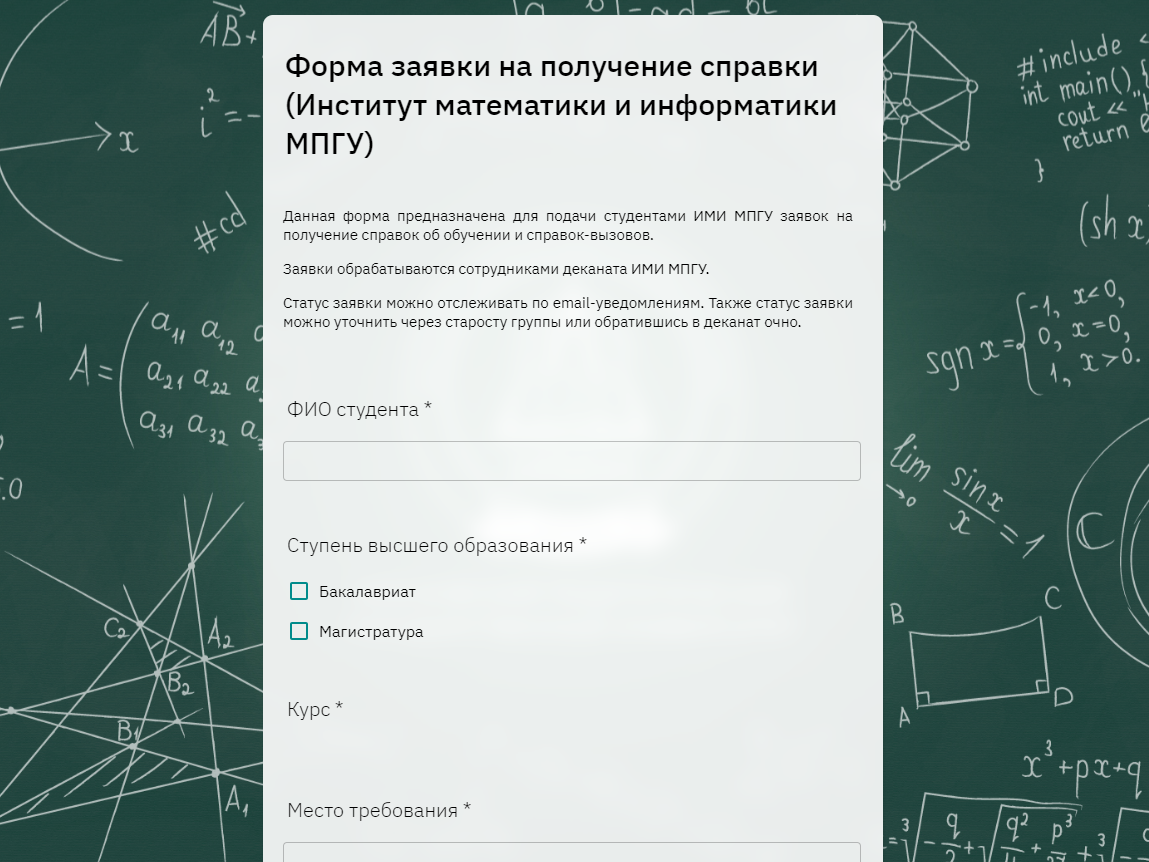
\includegraphics[width=0.69\textwidth]{images/screenshot.png}
	\caption{Форма заявки на получение справки}
	\label{fig:inquiries_form}
\end{figure}

Кроме того, в~документ~TeX можно вставлять и другие PDF документы (рис.~\ref{fig:idef0_p2}~и~\ref{fig:idef0_p3}).

\begin{figure}[!p]
	\centering
	\vspace{-1em}
	\hspace*{-25pt}\includegraphics[page=2, width=1.05\textwidth]{images/idef0.pdf}
	\vspace*{-2.25em}
	\caption{Диаграмма IDEF0. Узел A0 <<Работа дирекции ИМИ МПГУ>>}
	\label{fig:idef0_p2}
\end{figure}

\begin{figure}[!p]
	\centering
	\vspace{-1em}
	\hspace*{-12pt}\includegraphics[page=3, width=1.05\textwidth]{images/idef0.pdf}
	\vspace*{-2.25em}
	\caption{Диаграмма IDEF0. Узел A1 <<Работа с информацией\linebreak о студентах>>}
	\label{fig:idef0_p3}
\end{figure}

\newpage

Можно расставить несколько рисунков в~линию:

\begin{figure}[!h]
	\centering
	\begin{minipage}{0.32\textwidth}
		\centering
		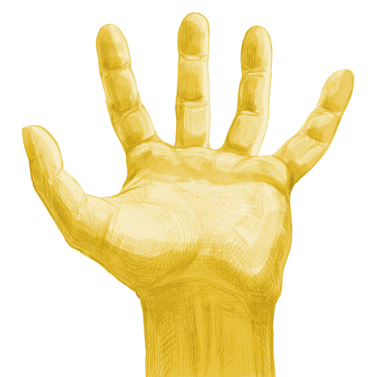
\includegraphics[height=100pt]{images/totum-logo.png}
		\caption{Логотип Totum}
		\label{fig:totum_logo}
	\end{minipage}
	\begin{minipage}{0.32\textwidth}
		\centering
		
\includegraphics[height=100pt]{images/1c-logo.jpg}
		\caption{Логотип\linebreak 1С: Предприятие}
		\label{fig:1c_logo}
	\end{minipage}
	\begin{minipage}{0.32\textwidth}
		\centering
		
\includegraphics[height=100pt]{images/phpmaker-logo.png}
		\caption{Логотип PHPMaker}
		\label{fig:phpmaker_logo}
	\end{minipage}
\end{figure}

Вставим в~работу также длинную таблицу (таблица~\ref{table:devinstrum_comp}).

\begin{table}[!h]
	\begin{center}
		\caption{Сравнительный анализ средств разработки}
		\label{table:devinstrum_comp}
	\end{center}
\end{table}\vspace*{-3.2em}

{\small\begin{longtable}{|>{\arraybackslash}p{90pt}|>{\arraybackslash}p{110pt}|>{\arraybackslash}p{110pt}|>{\arraybackslash}p{110pt}|}
		\hline
		\centering \textbf{Критерии} & \centering \textbf{Totum} & \centering \textbf{1С: Предприятие} &  \hfil\textbf{PHPMaker}\hfil \\
		\hline
		\endfirsthead
		\multicolumn{4}{r}{\fontsize{14}{16.8}\selectfont\textit{Продолжение таблицы}} \\
		\hline
		\centering \textbf{Критерий} & \centering \textbf{Totum} & \centering \textbf{1С: Предприятие} &  \hfil\textbf{PHPMaker}\hfil \\
		\hline
		\endhead
		\multicolumn{4}{|c|}{\textbf{\textit{Характеристики средства разработки}}} \\
		\hline
		Языки\newline разработки & Totum-код & Встроенный язык \mbox{программирования 1С} & PHP, HTML, CSS, SQL \\
		\hline
		Написание\newline запросов к базе данных & Опосредованное & Опосредованное & Непосредственное \\
		\hline
		Язык интерфейса & Русский, английский и другие & Русский, английский и другие & Английский \\
		\hline
		Исходный код & Открытый & Закрытый & Закрытый \\
		\hline
		Лицензия & Свободная & Проприетарная & Проприетарная \\
		\hline
		Цена & Бесплатно & Клиентская лицензия~--- от 7\,000 руб.; серверная лицензия~--- от 55\,500 руб. & От 379,95 долларов США \\
		\hline
		\multicolumn{4}{|c|}{\textbf{\textit{Возможные характеристики разрабатываемой информационной системы}}} \\
		\hline
		Клиент & Веб-интерфейс & Толстый и тонкий клиенты для ОС Windows, macOS, Linux; веб-интерфейс & Веб-интерфейс \\
		\hline
		Работа на\newline мобильных устройствах & Адаптированный веб-интерфейс & Мобильное приложение для Android и iOS & Неадаптированный веб-интерфейс \\
		\hline
		Серверная операционная система & Linux & Linux, Windows & Linux, Windows \\
		\hline
		База данных & PostgreSQL & \mbox{PostgreSQL, Microsoft} SQL, Oracle Database и другие & MySQL, PostgreSQL, Microsoft SQL, Oracle Database и SQLite \\
		\hline
\end{longtable}}\vspace*{-0.21em}
\setcounter{table}{\numexpr\value{table}-1}